\section{Results}\label{results}

\subsection{Case study: the central room in six rounds}\label{case-study-the-central-room-in-six-rounds}

The hub is the middle module of the Moon base, where the walkway tubes meet: a twelve-sided shell over a sunken pit, with four tube hatches and an airlock. Its structure came from a cutaway the owner picked from twenty drawn by a picture model from reference pictures he kept (Figure 1). It was then rebuilt six times between 6 and 7 October 2026, each round answering what the owner found in the last. Table 3 gives the rounds; the numbers are from the build logs.

\begin{figure}
\centering
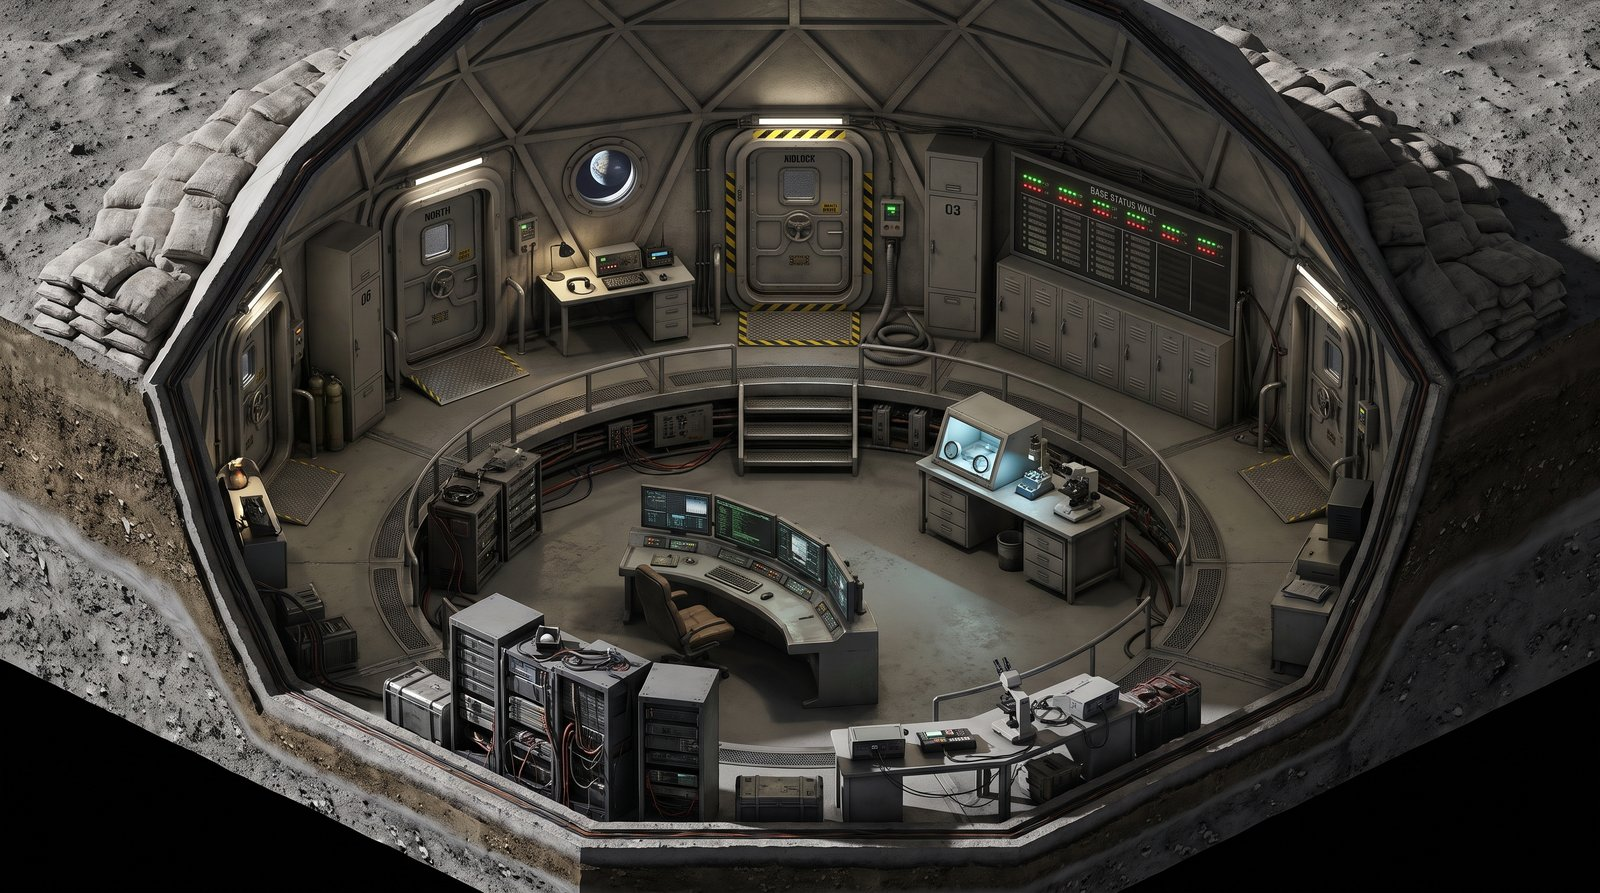
\includegraphics[width=0.9\linewidth,height=\textheight,keepaspectratio,alt={The picked concept for the hub, cutaway C12: a twelve-sided shell over a sunken pit. Drawn by Nano Banana Pro from reference pictures the owner kept; picked by the owner from twenty cutaways. This picture fixes the room's structure; it is not shipped.}]{figures/hub-concept-c12.jpg}
\caption{The picked concept for the hub, cutaway C12: a twelve-sided shell over a sunken pit. Drawn by Nano Banana Pro from reference pictures the owner kept; picked by the owner from twenty cutaways. This picture fixes the room's structure; it is not shipped.}
\end{figure}

\textbf{Table 3.} The hub's six rounds. Cost is rented GPU time (€) and picture-model calls (\$). Frame time is the mean on the RTX 5080 at night, 1600×900.

{\def\LTcaptype{none} % do not increment counter
\begin{longtable}[]{@{}
  >{\raggedright\arraybackslash}p{(\linewidth - 8\tabcolsep) * \real{0.2000}}
  >{\raggedright\arraybackslash}p{(\linewidth - 8\tabcolsep) * \real{0.2000}}
  >{\raggedright\arraybackslash}p{(\linewidth - 8\tabcolsep) * \real{0.2000}}
  >{\raggedright\arraybackslash}p{(\linewidth - 8\tabcolsep) * \real{0.2000}}
  >{\raggedright\arraybackslash}p{(\linewidth - 8\tabcolsep) * \real{0.2000}}@{}}
\toprule\noalign{}
\begin{minipage}[b]{\linewidth}\raggedright
Round
\end{minipage} & \begin{minipage}[b]{\linewidth}\raggedright
What changed
\end{minipage} & \begin{minipage}[b]{\linewidth}\raggedright
Owner's verdict
\end{minipage} & \begin{minipage}[b]{\linewidth}\raggedright
Cost
\end{minipage} & \begin{minipage}[b]{\linewidth}\raggedright
Frame time
\end{minipage} \\
\midrule\noalign{}
\endhead
\bottomrule\noalign{}
\endlastfoot
1 (slice of two walls, A/B) & surface library (11 surfaces), sorter by shape, room checks, PartCrafter parts & blind pick for the new route: ``Y looks much cleaner'' & €0.88, \$0 & 7.81 ms against 7.53 (whole hub, one slice changed) \\
2 (slice, A/B) & library to 71 variants, screens and labels as code parts, roof check, shared texture sets & blind pick for the new route again & €1.70, \$0 & 8.05 ms against 8.24 \\
3 (whole hub) & the route end to end: 74 models, 457 pieces & a move made without asking; 26 old models still showing; Chinese labels; floor fittings ``smacked on'' & €1.67 with its fix round, \$0 & 6.78 ms (old hub 9.22) \\
4 (whole hub) & code only for plain plates, pipes and trims; detail through the pipeline with the picture's own colours laid over & detail back, but ``pretty much all of this became messy'', ``inconsistent with the rest of the room'' & €8.50, \$5.09 & 9.6 ms \\
5 (eight pieces, blind A/B) & method B: shape only from the pipeline, every surface from the library, code or pipeline by the parts check & B wins for the door, notice board and porthole; tool board, locker and console still wrong & €0.21, \$0 & not run \\
6 (whole hub) & method B everywhere; composites split, one model per object; straightness check & ``this looks amazing, I have no negative feedback'' & about €3.48, \$1.07 & 5.6 ms (round four 9.6) \\
\end{longtable}
}

Three findings come out of the six rounds.

\textbf{Grounded checks catch what an agent misses, and miss what only play shows.} Already in round one the room checks found the faults the owner had seen in the old hub: light escaping through walls and roof fell from 1.53 percent of 5,817 rays to zero, a box that covered the porthole was moved 0.5 m by the placement check, and in round two the surface check found all nine roof pieces the owner had seen hanging below the roof. Colour noise inside each surface fell from a median of 31.1 to 3.2 percent. But the checks did not find what the owner found by walking the room in round three: that 26 old models were still showing, because the claim ``every piece is made'' had covered only the kit and not what the engine actually loaded. A check that walks the loaded scene (the made-only check) was added, and found 26 before the fix and none after.

\textbf{The split between code and pipeline is the hard decision, and a list does not make it.} Round three routed by shape and sent the furniture to code, and the owner found the old pieces' detail gone. Round four answered with an allow-list (code only for 19 plain kinds) and laid each picture's own colours over the library surfaces; the detail came back, but every piece brought its own rust and stains, and the room read as messy. Round five replaced the list with the parts check and took the picture's colours away entirely; the owner's blind picks favoured that method wherever its pieces were built well, and the three that still failed had one thing in common: each was a set of objects generated as one model, or a box the picture-to-3D model could not keep straight. Round six answered with one model per object and the straightness check (the round-four locker leaned 13 degrees; a generated radio 11, so it moved to code). Figure 2 shows the tool board in rounds four and six.

\begin{figure}
\centering
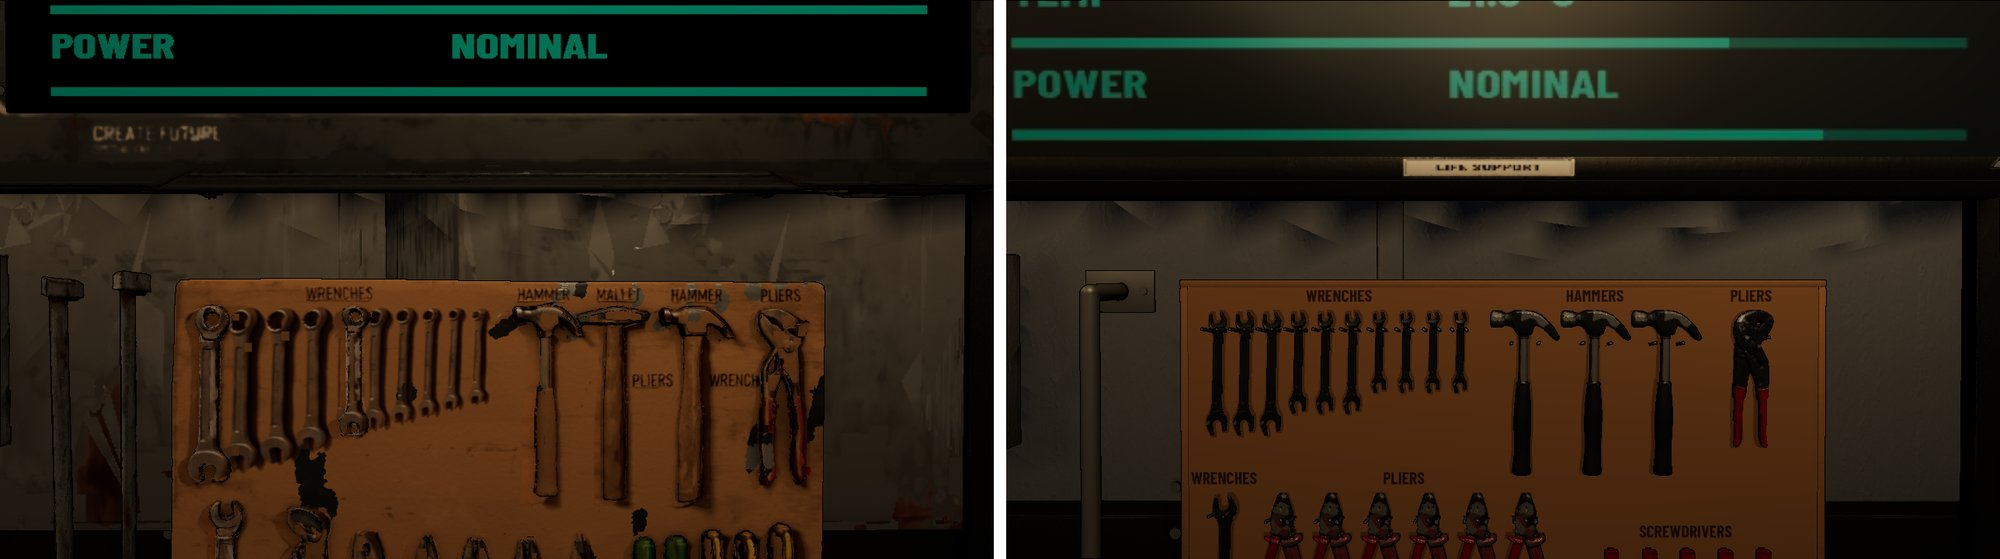
\includegraphics[width=1\linewidth,height=\textheight,keepaspectratio,alt={The hub's tool board up close in round four (left) and round six (right), same camera and build. Left: one generated model with the picture's own colours laid over the library surfaces. Right: a code-built board with outlines printed from each tool's silhouette and 26 tools, each its own model, with library surfaces only. In-game shots from 2099.}]{figures/hub-toolboard-r4-r6.jpg}
\caption{The hub's tool board up close in round four (left) and round six (right), same camera and build. Left: one generated model with the picture's own colours laid over the library surfaces. Right: a code-built board with outlines printed from each tool's silhouette and 26 tools, each its own model, with library surfaces only. In-game shots from 2099.}
\end{figure}

\textbf{Consistency and cost moved together.} Round six's room drew 0.45 million triangles against round four's 1.96 million, ran at 5.6 ms a frame against 9.6, and took 187 MB on disk against 487. The gain came from shared texture sets, triangles set by an object's size, and code builders for the room's fittings. Small objects need a floor: at the first size budget the pliers' outline went angular up close, so every small generated object now gets at least 5,000 triangles.

Over the six rounds the hub's route cost about €16.44 of rented GPU time and \$6.16 of picture calls, and took about 23 hours of wall-clock time. \textcolor{red}{[TODO: Wall time per round is read from first and last log lines and includes waiting; an exact figure needs the logs re-read]}. The concept stage before round one (twenty cutaways, the owner's pick) is not included.

\subsection{World 1, place by place}\label{world-1-place-by-place}

After the hub was signed off, round six's method became the route for every place, and the rest of world 1 was built in parallel, about one agent per place, between 7 October evening and 8 October noon, when the owner paused the game work. Table 4 is the per-place record the agents kept.

\textbf{Table 4.} Time, cost and models per place for world 1 after the hub. Wall time includes waiting for cloud machines, quota resets and two usage-limit stops; several places shared one agent, and a shared time or cost is marked. Costs are floors from the agents' own notes, not reconciled with the cloud bill. Models are counted as built in code / made through the prop pipeline.

{\def\LTcaptype{none} % do not increment counter
\begin{longtable}[]{@{}
  >{\raggedright\arraybackslash}p{(\linewidth - 8\tabcolsep) * \real{0.2000}}
  >{\raggedright\arraybackslash}p{(\linewidth - 8\tabcolsep) * \real{0.2000}}
  >{\raggedright\arraybackslash}p{(\linewidth - 8\tabcolsep) * \real{0.2000}}
  >{\raggedright\arraybackslash}p{(\linewidth - 8\tabcolsep) * \real{0.2000}}
  >{\raggedright\arraybackslash}p{(\linewidth - 8\tabcolsep) * \real{0.2000}}@{}}
\toprule\noalign{}
\begin{minipage}[b]{\linewidth}\raggedright
Place
\end{minipage} & \begin{minipage}[b]{\linewidth}\raggedright
Wall time (min)
\end{minipage} & \begin{minipage}[b]{\linewidth}\raggedright
Cloud €
\end{minipage} & \begin{minipage}[b]{\linewidth}\raggedright
Pictures \$
\end{minipage} & \begin{minipage}[b]{\linewidth}\raggedright
Code / pipeline
\end{minipage} \\
\midrule\noalign{}
\endhead
\bottomrule\noalign{}
\endlastfoot
Moon ground, whole Moon (round two) & 360 & 0.08 & 5.29 & 0 / 0 \\
Old station & 253, shared with the wreck & 4.93 & 3.22 & 10 / 14 \\
Wreck & shared & 2.40 & 2.68 & 3 / 13 \\
Lab, round one & 367 & 5.55 & 2.68 & 53 / 14 \\
Lab, round two (not shipped) & --- & 2.30 & 1.47 & 54 / 22 \\
Workshop & 519 & 2.80 & 3.35 & 110 / 8 \\
Greenhouse & 990 & 4.60 & 2.13 & 157 / 3 \\
Crew habitat & 530, shared by three & 1.31 & 1.34 & 108 / 2 \\
Airlock & shared & 0.79 & 0.13 & 81 / 1 \\
Walkway tubes & shared & 0.14 & 0 & 25 / 0 \\
Prologue flat with balcony & 633, shared by two & 4.69 for both & 2.41 for both & 35 / 10 \\
Prologue stairwell & shared & shared & shared & 44 / 1 \\
Street (not shipped) & 1039, shared by three & 1.42 & 1.74 & 45 / 2 \\
Square (not shipped) & shared & 2.05 & 1.07 & 75 / 2 \\
Launch view (not shipped) & shared & 0.75 & 0.40 & 4 / 1 \\
Mars ground & 513 & 0.64 & 1.58 & 0 / 0 \\
Mars camp grounds, two parts & 271 + 280 & 2.05 + 0.77 & 1.04 + 0.27 & 2 / 8 \\
Mars camp habitat, two passes & 586 + 445 & 5.20 + 1.60 & 1.21 + 0 & 59 / 5 \\
Garage and hangar (paused) & --- & about 2.60 & 8.71 & --- \\
\textbf{Total, 21 rows} & & \textbf{46.67} & \textbf{40.72} & \textbf{865 / 106} \\
\end{longtable}
}

Two things stand out. First, the cost of a place is small next to the time it takes: most places cost a few euros of GPU time and a few dollars of pictures, while their wall time ran to many hours, mostly waiting. Second, the route leaned heavily on code: 865 of 971 models were code builders. In some rooms that gave clean, convincing pieces (the greenhouse's console, tank and racks are all code), but in the lab the same pull gave plain and sparse results, and the owner's view is that code builders are clean but neither scale nor are robust.

\textbf{The Moon's ground, the old station and the wreck.} The ground round the base is planned rather than seeded: a dimensioned plan in code, a diorama picture, plan heights following it, a skin painted over the plan, fine relief from Depth Anything V2 Small, and boulders from Pixal3D. Its first round holds 11 named craters of 9 kinds and 140 small ones round the base's flats and paths; the owner preferred it to a crater generated with Infinigen (``new is a lot better''), but that comparison was not blind, because the two were drawn in different renderers and he could tell them apart in every view. Round two planned the whole Moon over the six faces of a cube, with 27 named far craters, about 1,300 small ones and 7,000 rocks, and blended the faces so the median step at an edge fell from 0.48 m to 0.02 m. It also found an old bug that had flattened every crater rim. The old station and the wreck were built on the signed-off route (Figures 3 and 4); the owner signed both off on first sight (``it just looks great'').

\begin{figure}
\centering
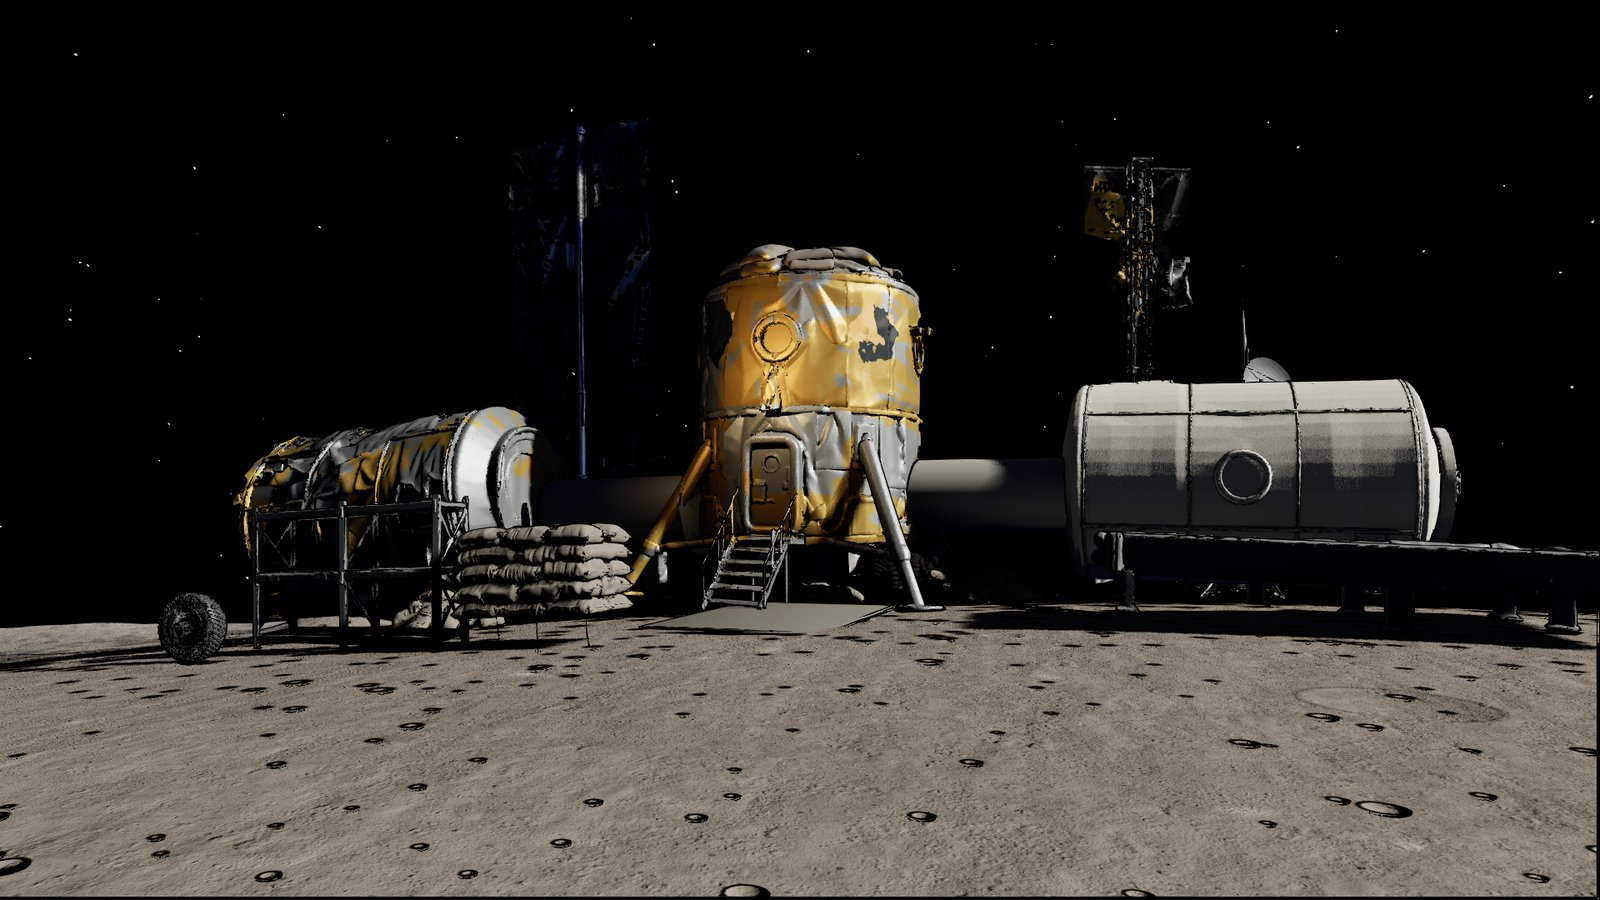
\includegraphics[width=1\linewidth,height=\textheight,keepaspectratio,alt={The old station on the Moon: a lived-in lander joined by walkway tubes to a torn first module and a shut lab, with sandbags, masts and a radiator. 14 objects through the prop pipeline and 10 plain pieces in code, on the planned ground. In-game shot from 2099.}]{figures/old-station.jpg}
\caption{The old station on the Moon: a lived-in lander joined by walkway tubes to a torn first module and a shut lab, with sandbags, masts and a radiator. 14 objects through the prop pipeline and 10 plain pieces in code, on the planned ground. In-game shot from 2099.}
\end{figure}

\begin{figure}
\centering
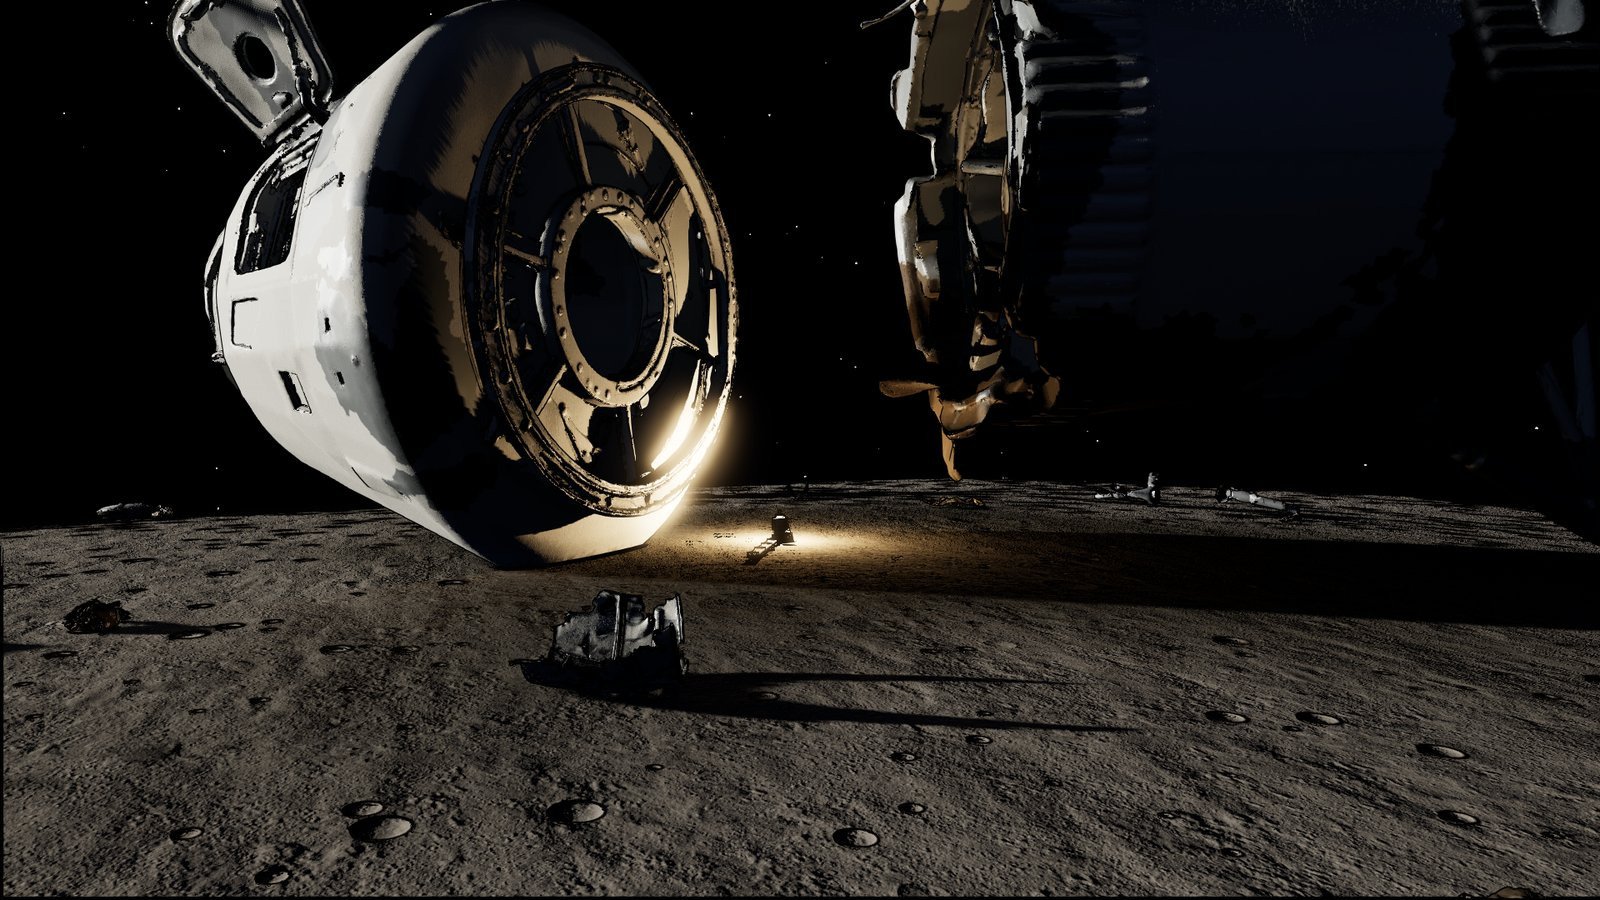
\includegraphics[width=1\linewidth,height=\textheight,keepaspectratio,alt={The wreck: a rocket broken in two with a work lamp burning in the break. 13 objects through the prop pipeline and 3 code-built cables. In-game shot from 2099.}]{figures/wreck.jpg}
\caption{The wreck: a rocket broken in two with a work lamp burning in the break. 13 objects through the prop pipeline and 3 code-built cables. In-game shot from 2099.}
\end{figure}

\textbf{Base modules, prologue and Mars.} The habitat, airlock and walkway tubes, the lab, workshop and greenhouse were pushed with their checks green; the owner's in-game test of them is \textcolor{red}{[TODO: pending]}. The owner judged the lab's first build to have ``lost a massive amount of detail'' against its concept; that gave the route its concept-density check, and the lab's second round, mapped element by element to its concept, was not finished before the pause. The prologue's flat and stairwell were pushed; its street, square and launch view were built but not pushed, because one scene-check finding was still open. On Mars, the ground round the camp and the camp's two habitat domes were pushed; the domes were first built larger than their concepts (13.9 and 11.4 m across against about 10 and 9 m) and read sparser, so they were shrunk to the concepts' size; the camp grounds still fail the density check while five close-ups wait for the picture quota.

\textbf{Sound.} Every sound the game names, 61 in all, was generated in one batch: 244 takes in 123 minutes on one rented L4 for €1.61, each chosen by its prompt match less measured faults. The owner listened and kept most of them, but went back to earlier recordings for breathing in the helmet, the sliding door and footsteps on steel. A prompt-match score did not foresee that.

\textbf{Faults caught, before and after spending.} Every place recorded the faults its checks caught before money was spent and those found afterwards. Typical faults caught before spending were labels voted onto the wrong material by a dusty picture (one lander came out 98 percent sandbag), walls under 3 mm, a torn leg 2.4 m long against a 1.4 m piece limit, close-ups that drew the whole room instead of one object, and a door in a partition one could walk around. Typical faults found afterwards were pieces standing up where they should lie (an apron as a 4 m wall, cables as fences), shots taken at night because a Martian day is longer than the bench assumed, and rooms sparser than their concepts. \textcolor{red}{[TODO: A count of faults per check, before and after spend, over all places needs the free-text columns of the scaling table coded by hand]}.

\subsection{What failed, and why}\label{what-failed-and-why}

\begin{itemize}
\tightlist
\item
  \textbf{Patchy surfaces from picture colours.} Choosing each face's surface by its picture colour lets shade and shadow flip faces between surfaces, which bakes as dark blotches. Parts as the painting unit, one surface per part with the picture only choosing which, is the fix; it was being built when the work paused.
\item
  \textbf{Sparse rooms.} Built rooms read sparser than their concepts: inventories kept the main objects and dropped the wall equipment, and a concept shows only two or three walls. The concept-density check catches it; the world step is meant to fill the walls a concept does not show, and is untested here.
\item
  \textbf{Quotas, not compute, set the pace.} The picture model's shared daily cap (250 pictures) ran out within half an hour of its reset more than once, and close-ups waited overnight; GPU stock ran out in every zone at least once.
\item
  \textbf{The agents' own errors.} An agent moved the console without asking; a claim that every piece was made was false; one blind page was not blind. Each became a rule or a check, but each first cost a round of the owner's attention.
\end{itemize}
